% \documentclass[aspectratio=169,notes]{beamer}
\documentclass[aspectratio=169]{beamer}
\usetheme[faculty=phil]{fibeamer}
\usepackage{polyglossia}
\setmainlanguage{english} %% main locale instead of `english`, you
%% can typeset the presentation in either Czech or Slovak,
%% respectively.
\setotherlanguages{russian} %% The additional keys allow
%%
%%   \begin{otherlanguage}{czech}   ... \end{otherlanguage}
%%   \begin{otherlanguage}{slovak}  ... \end{otherlanguage}
%%
%% These macros specify information about the presentation
\title[Introduction to Robotics (In2Ro)]{Introduction to Robotics, Homework Hard 2} %% that will be typeset on the
\subtitle{Mobile robots: JetBot, Scout 2, Limo CoRoT 
\\ Odometry calibration and parking in a pose \\ \ } %% title page.
\author{Oleg Bulichev}
%% These additional packages are used within the document:
\usepackage{ragged2e}  % `\justifying` text
\usepackage{booktabs}  % Tables
\usepackage{tabularx}
\usepackage{tikz}      % Diagrams
\usetikzlibrary{calc, shapes, backgrounds, trees, positioning, arrows.meta}
\usetikzlibrary{decorations.pathreplacing,calligraphy,calc,graphs}
\usepackage{amsmath, amssymb}
\usepackage{url}       % `\url`s
\usepackage{listings}  % Code listings
\usepackage{floatrow}
\usepackage{subcaption}
\usepackage{mathtools}
\usepackage{todonotes}
\usepackage{fontspec}
\usepackage{multicol}
\usepackage{pdfpages}
\usepackage{wrapfig}
\usepackage{qrcode}
\usepackage{animate}
\usepackage{booktabs}
\usepackage{multirow}
\usepackage{graphicx}
\usepackage{colortbl}

\graphicspath{{resources/}}
\frenchspacing

\setbeamertemplate{caption}{\raggedright\insertcaption\par}
\usetikzlibrary{graphs}

% \usepackage[backend=biber,style=ieee,autocite=footnote]{biblatex}
% \addbibresource{biblio.bib}
% \DefineBibliographyStrings{english}{%
%   bibliography = {References},}

\newcommand{\oleg}[2][] {\todo[color=red, #1] {OLEG:\\ #2}}
\newcommand{\fbckg}[1]{\usebackgroundtemplate{\includegraphics[width=\paperwidth]{#1}}}%frame background

\usepackage[framemethod=TikZ]{mdframed}
\newcommand{\dbox}[1]{
\begin{mdframed}[roundcorner=3pt, backgroundcolor=yellow, linewidth=0]
\vspace{1mm}
{#1}
\vspace{1mm}
\end{mdframed}
}

\begin{document}
\setlength{\abovedisplayskip}{0pt}
\setlength{\belowdisplayskip}{0pt}
\setlength{\abovedisplayshortskip}{0pt}
\setlength{\belowdisplayshortskip}{0pt}

\fbckg{fibeamer/figs/title_page.png}
\frame[c]{\setcounter{framenumber}{0}
    \usebeamerfont{title}%
    \usebeamercolor[fg]{title}%
    \begin{minipage}[b][6.5\baselineskip][b]{\textwidth}%
        \textcolor{black}{\raggedright\inserttitle}
    \end{minipage}
    % \vskip-1.5\baselineskip

    \usebeamerfont{subtitle}%
    \usebeamercolor[fg]{framesubtitle}%
    \begin{minipage}[b][3\baselineskip][b]{\textwidth}
        \raggedright%
        \insertsubtitle%
    \end{minipage}
    \vskip.25\baselineskip
}

\fbckg{fibeamer/figs/common.png}

\begin{frame}[t]{What this homework is}
\framesubtitle{Teach a mobile robot to know where it is and to stop where you ask}
    A mobile robot estimates its pose from its wheels, and that estimate is wrong in a way
    that depends on the particular robot. You measure that error, correct it, and then
    use the corrected estimate to drive into a marked parking rectangle.
    \medskip

    \begin{itemize}
        \item Choose \textbf{one} robot: JetBot (write its number, 1--5), Scout 2, or Limo CoRoT.
        \item Name the robot on the first page of your report.
        \item If you chose the Limo arm in Homework Hard 1, use Limo here as well.
    \end{itemize}
    \medskip

    The task is stated at a high level. How to do each step, and why it works, is for you
    to work out and to describe in the report.
\end{frame}

\begin{frame}[t]{Four tasks, one chain}
\framesubtitle{Each task produces the input of the next one}
    \centering
    \vspace{2mm}
    \begin{tikzpicture}[
        box/.style={draw, rounded corners=3pt, minimum width=3.0cm, minimum height=1.4cm,
                    align=center, fill=blue!8},
        arr/.style={-{Stealth[length=2.5mm]}, thick}]
        \node[box] (a) {Task 1\\ Odometry};
        \node[box, right=5mm of a] (b) {Task 2\\ Square test\\ and correction};
        \node[box, right=5mm of b] (c) {Task 3\\ Reach\\ a pose};
        \node[box, right=5mm of c] (d) {Task 4\\ Open loop\\ for comparison};
        \draw[arr] (a) -- (b);
        \draw[arr] (b) -- (c);
        \draw[arr] (c) -- (d);
    \end{tikzpicture}
    \medskip

    \begin{minipage}{0.92\textwidth}
        \raggedright
        Odometry (Task 1) is corrected in Task 2 and then feeds the controller of Task 3.
        Task 4 drives the same goal without any feedback, so you can see what the
        feedback bought you.
    \end{minipage}
\end{frame}

\begin{frame}[t]{JetBot (units 1--5)}
    \begin{minipage}[t]{0.55\textwidth}
        \vspace{0pt}
        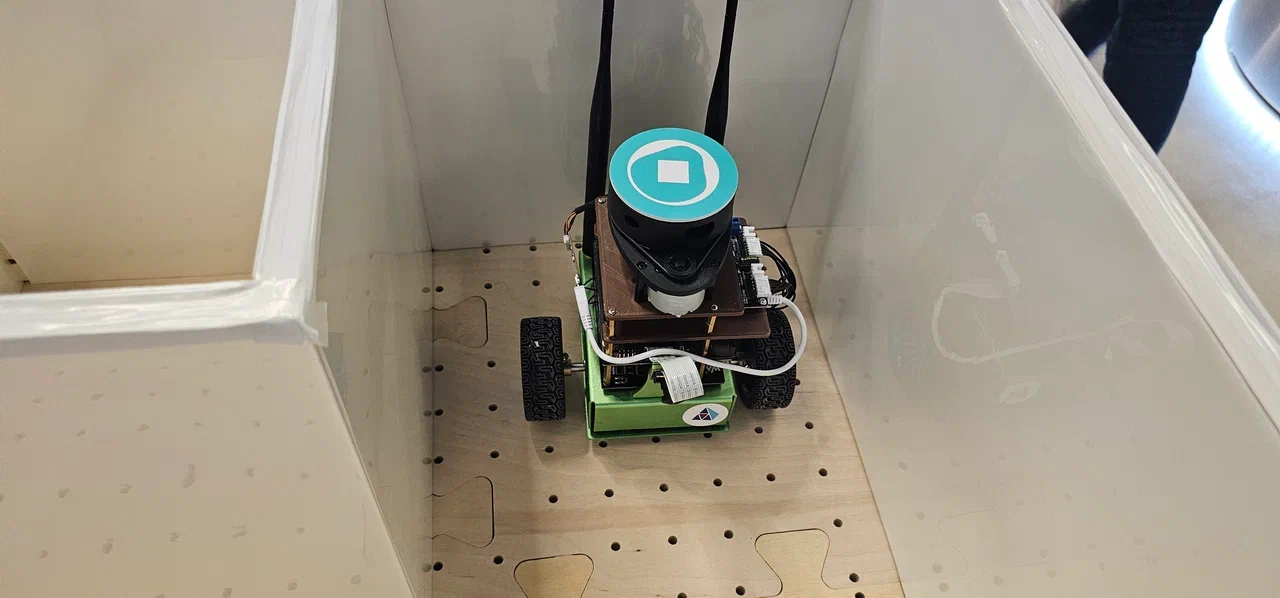
\includegraphics[width=\linewidth]{robot_jetbot.png}
    \end{minipage}
    \hfill
    \begin{minipage}[t]{0.43\textwidth}
        \vspace{0pt}
        \small
        \textbf{What it is.} A small differential-drive robot: two driven wheels and a caster.
        Each wheel has an encoder with 1760 counts per revolution. The motor board is on a USB
        serial port. Nominal wheel radius 0.033\,m, wheel track 0.15\,m.
        \smallskip

        \textbf{Your JetBot number.} Set \texttt{ROBOT\_ID} to it; every log carries it.
        \smallskip

        \textbf{Documentation.} The header of \texttt{jetbot\_hw.py}.
    \end{minipage}
\end{frame}

\begin{frame}[t]{Scout 2 (AgileX)}
    \begin{minipage}[t]{0.27\textwidth}
        \vspace{0pt}
        \centering
        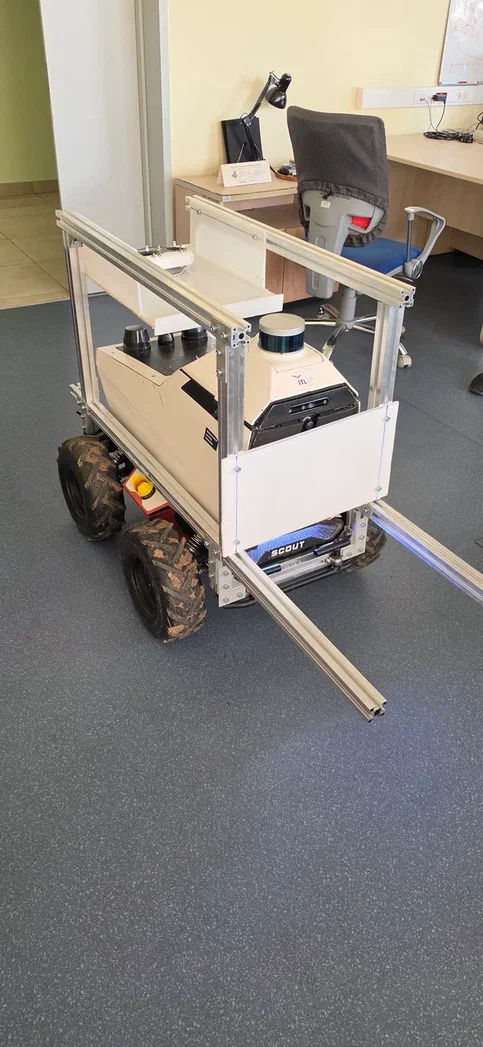
\includegraphics[height=5.6cm,width=\linewidth,keepaspectratio]{robot_scout.png}
    \end{minipage}
    \hfill
    \begin{minipage}[t]{0.70\textwidth}
        \vspace{0pt}
        \small
        \textbf{What it is.} A four-wheel skid-steer outdoor robot: it turns by driving the
        left and right wheels at different speeds, and the wheels slip while it turns. Our unit
        carries a frame and a lidar that this homework does not use.
        \smallskip

        \textbf{Control.} Over a CAN bus with the \texttt{ugv\_sdk} library; it reports its
        own linear and angular velocity. See \texttt{scout\_hw.py}. Keep the remote controller in
        your hand and the area free.
        \smallskip

        \textbf{Documentation.} \url{github.com/westonrobot/ugv_sdk}; the SCOUT 2.0 user manual.
    \end{minipage}
\end{frame}

\begin{frame}[t]{Limo CoRoT (AgileX), Ackermann mode}
    \begin{minipage}[t]{0.27\textwidth}
        \vspace{0pt}
        \centering
        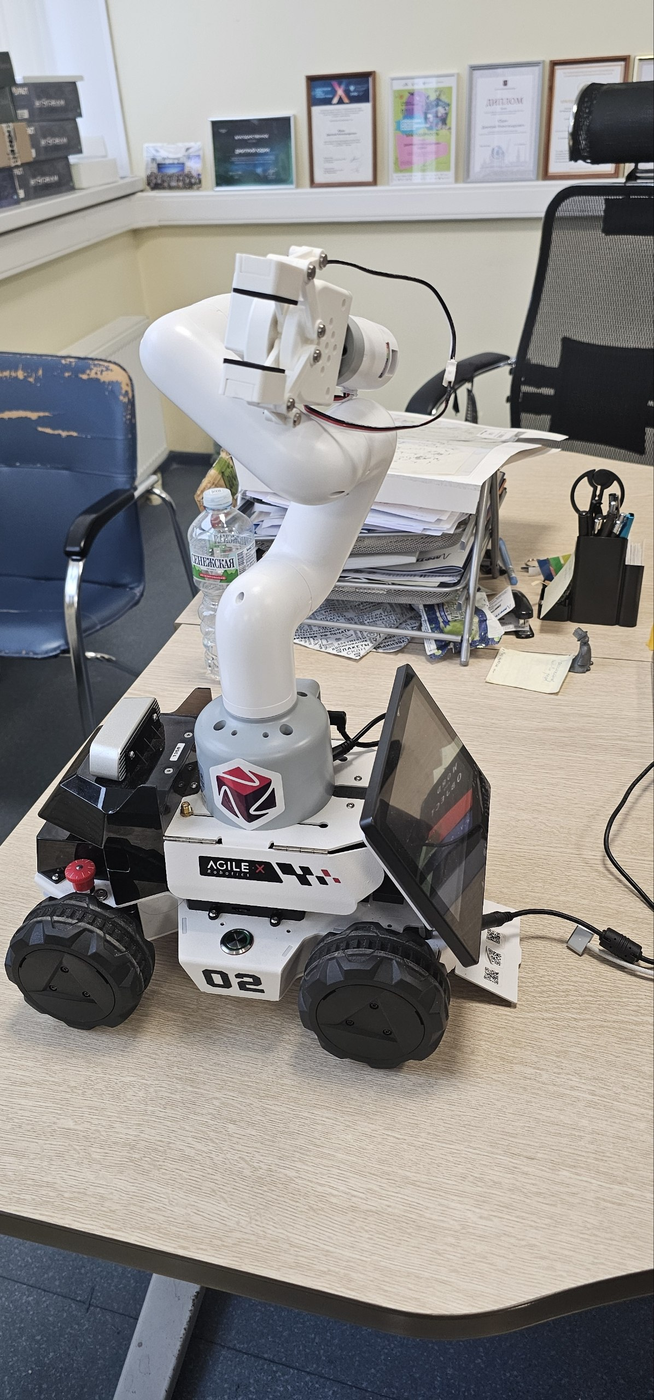
\includegraphics[height=5.6cm,width=\linewidth,keepaspectratio]{robot_limo.png}
    \end{minipage}
    \hfill
    \begin{minipage}[t]{0.70\textwidth}
        \vspace{0pt}
        \small
        \textbf{What it is.} A four-wheel car-like robot with a steered front axle (Ackermann
        steering). It cannot turn on the spot: its turning radius has a minimum.
        \smallskip

        \textbf{Control.} Through the \texttt{pylimo} Python library over a serial port: a
        speed command and a steering angle; it reports its speed and steering angle. See
        \texttt{limo\_hw.py}. Put the robot in Ackermann mode first.
        \smallskip

        \textbf{Documentation.} \url{pypi.org/project/pylimo}; \url{github.com/agilexrobotics/limo_ros2}
        for the ROS option.
    \end{minipage}
\end{frame}

\begin{frame}[t]{Starter files}
\framesubtitle{All of it runs without ROS; ROS is allowed}
    \small
    \begin{center}
    \begin{tabular}{@{}lll@{}}
        \toprule
        File & Robot & What it gives you \\
        \midrule
        \texttt{jetbot\_hw.py} & JetBot & encoder ticks, wheel speed commands \\
        \texttt{scout\_hw.py}  & Scout 2 & reported velocity, velocity commands \\
        \texttt{limo\_hw.py}   & Limo & reported speed and steering, drive command \\
        \texttt{hw\_log.py}    & all & CSV log whose first line names the robot \\
        \bottomrule
    \end{tabular}
    \end{center}
    \smallskip

    Each file prints the robot's state for three seconds when you run it. Nothing in them
    knows the true wheel radius, track or wheelbase of your robot: finding the corrections
    is Task 2.
\end{frame}

\begin{frame}[t]{Task 1: Odometry}
\framesubtitle{From wheel motion to the pose $(x, y, \theta)$}
    Pose = position $(x, y)$ and heading $\theta$ of the robot in a frame fixed to the floor.
    \begin{itemize}
        \item \textbf{Differential drive, encoders (JetBot):} tick increments $\Delta N_L,\Delta N_R$ give wheel paths
              $\Delta s_{L,R} = 2\pi r\,\Delta N_{L,R}/\mathrm{CPR}$ ($r$ wheel radius,
              CPR counts per revolution). Then $\Delta s = (\Delta s_R+\Delta s_L)/2$,
              $\Delta\theta = (\Delta s_R-\Delta s_L)/b$ ($b$ wheel track).
        \item \textbf{Skid-steer, reported velocity (Scout 2):} integrate the reported $v$ (linear) and $\omega$ (angular).
        \item \textbf{Ackermann, reported speed and steering (Limo):} integrate $\dot x = v\cos\theta$, $\dot y = v\sin\theta$,
              $\dot\theta = v\tan\delta / L$ with the reported speed $v$ and steering angle
              $\delta$; the wheelbase $L$ is yours to measure, and the scale of the reported
              steering angle is to be checked in Task 2.
    \end{itemize}
    Log everything with \texttt{hw\_log.py}.
\end{frame}

\begin{frame}[t]{Task 1: What to bring}
    \begin{itemize}
        \item Your odometry code and a plot of the path it computes for a short drive.
        \item The robot driven forward 2\,m: tape-measure distance against the odometry.
        \item The robot turned by a full revolution: what the odometry says.
    \end{itemize}
\end{frame}

\begin{frame}[t]{Task 2: Square test and correction}
\framesubtitle{Find out what the nominal numbers get wrong}
    Mark a $2\,\mathrm{m}\times2\,\mathrm{m}$ square on the floor with tape.
    \begin{itemize}
        \item Drive its four sides and four $90^\circ$ turns, first clockwise, then
              counter-clockwise, three runs each, by the odometry of Task 1.
        \item After each run measure with a tape how far the robot ended from where it
              started.
        \item From the two sets of errors estimate corrections to the wheel radius and the
              \emph{effective track} (the track that makes the turn angle right; on a skid-steer
              robot it is larger than the geometric one). Limo: the wheelbase and a steering factor.
        \item Apply the corrections and repeat.
    \end{itemize}
\end{frame}

\begin{frame}[t]{Task 2: What to bring}
    \begin{itemize}
        \item Photos of the taped square with the robot at the end of a run, tape in frame.
        \item A table of the end-point errors before and after the correction.
        \item The correction values and how you obtained them.
        \item Why the two directions of travel are needed.
    \end{itemize}
\end{frame}

\begin{frame}[t]{Task 3: Reach pose}
\framesubtitle{Same goal and same measurements for every robot}
    Goal pose $(x_g, y_g, \theta_g)$: park in a taped rectangle slightly larger than the robot.
    \begin{itemize}
        \item Drive the goal from the same start five times.
        \item After each run measure the position error and the heading error against the goal.
    \end{itemize}
    \medskip

    The only difference between robots is how the controller is written, because the wheels
    differ: a differential or skid-steer robot can turn on the spot, an Ackermann robot cannot.
    The next two frames give the controller of each drive type; use the one that fits your robot.
\end{frame}

\begin{frame}[t]{Task 3: Differential and skid-steer drive}
\framesubtitle{JetBot and Scout 2: feedback in polar coordinates}
    With $\rho$ the distance to the goal, $\alpha$ the angle between the robot heading and the
    line to the goal, and $\beta$ the angle between that line and the goal heading, the
    controller of lecture 8 is
    \[
        v = k_\rho\,\rho,\qquad \omega = k_\alpha\,\alpha + k_\beta\,\beta,
    \]
    stable for $k_\rho>0$, $k_\beta<0$, $k_\alpha-k_\rho>0$. Choose the gains inside these
    limits and test them.
\end{frame}

\begin{frame}[t]{Task 3: Ackermann drive}
\framesubtitle{Limo: an arc and a straight line}
    \begin{itemize}
        \item Measure the minimum turning radius: drive a full circle at the maximum steering
              angle and measure its diameter on the floor.
        \item Choose a goal that an arc followed by a straight line can reach (its final heading is
              then set by the arc; you may add a second arc). Follow the path by
              \emph{pure pursuit}: aim at the point of the path a distance $L_d$ ahead, at angle
              $\alpha$ from the heading, with steering $\delta=\arctan(2L\sin\alpha/L_d)$
              ($L$ the wheelbase).
    \end{itemize}
\end{frame}

\begin{frame}[t]{Task 3: What to bring}
    \begin{itemize}
        \item The gains (or $L_d$) and the reason for your choice.
        \item Five runs: a photo of the final position against the taped rectangle, and the
              measured position error and heading error of each run.
        \item Plots of the path the odometry recorded.
        \item Limo: the measured minimum turning radius.
    \end{itemize}
\end{frame}

\begin{frame}[t]{Task 4: Open loop for comparison}
\framesubtitle{The same goal, with no feedback}
    Compute from the nominal values a timed sequence of commands. JetBot and Scout 2: turn,
    drive straight, turn to the goal heading. Limo: it cannot turn on the spot, so a timed
    sequence of speed and steering commands along your arc and straight line. Send it blindly
    and run it five times from the same start.
    \begin{itemize}
        \item Measure the final position and heading errors as in Task 3.
        \item Compare the two sets of errors in one table.
    \end{itemize}
\end{frame}

\begin{frame}[t]{What you hand in}
\framesubtitle{The same rules for all four tasks}
    \textbf{One report.} The first page names your robot (JetBot with its number) and shows a
    photo of the setup. For each task:
    \begin{itemize}
        \item what you did and why, with the formulas and numbers;
        \item photos of the setup and the result, with a ruler or tape in frame wherever a
              distance is measured;
        \item screenshots of code, printed values and plots;
        \item a table of several runs, and what went wrong and what you changed.
    \end{itemize}
    Code goes as files; the report quotes only what it discusses.
\end{frame}

\fbckg{fibeamer/figs/last_page.png}
\frame[plain]{}

\end{document}
